Júlia gosta muito de animais domésticos.
 Ela tem vários cachorros, gatos, papagaios, mas seu animal preferido mesmo é sua formiga, que recebeu o nome de Fininha.


Aproveitando suas aulas de carpintaria, Júlia está construindo um brinquedo para Fininha.

Ela começou pegando dois pedaços de madeira de 1 metro cada um e construindo um degrau,
como mostra a figura abaixo:

\begin{figure}[h]
\begin{center}
  
\includegraphics[height=8em]{\CWD/degrau}
\end{center}
\end{figure}

Fininha sempre começa do ponto mais baixo do degrau, e sobe pelos segmentos do brinquedo até chegar ao topo.
 Mas ela não para por aí: ao chegar ao topo, Fininha começa a descer, depois sobe novamente, e assim segue, até ter fome.
 Nesse momento, a formiga fica sem energia e precisa se alimentar.
 Júlia, como boa dona, pega então alguns grãos de açúcar e leva até a boca de seu animal de estimação.


Para que o brinquedo fique menos monótono, Júlia decidiu transformar cada segmento do degrau em dois com metade do tamanho.
 Ela repetiu esse procedimento $K$ vezes.
 Cada vez que Júlia faz isso, o número de degraus do brinquedo dobra, e o tamanho de cada um dos novos segmentos fica exatamente metade do tamanho dos segmentos anteriormente.
 Na figura abaixo, você pode ver como o brinquedo ficou depois de uma, duas e três repetições desse procedimento.


\begin{figure}[h]
\begin{center}
  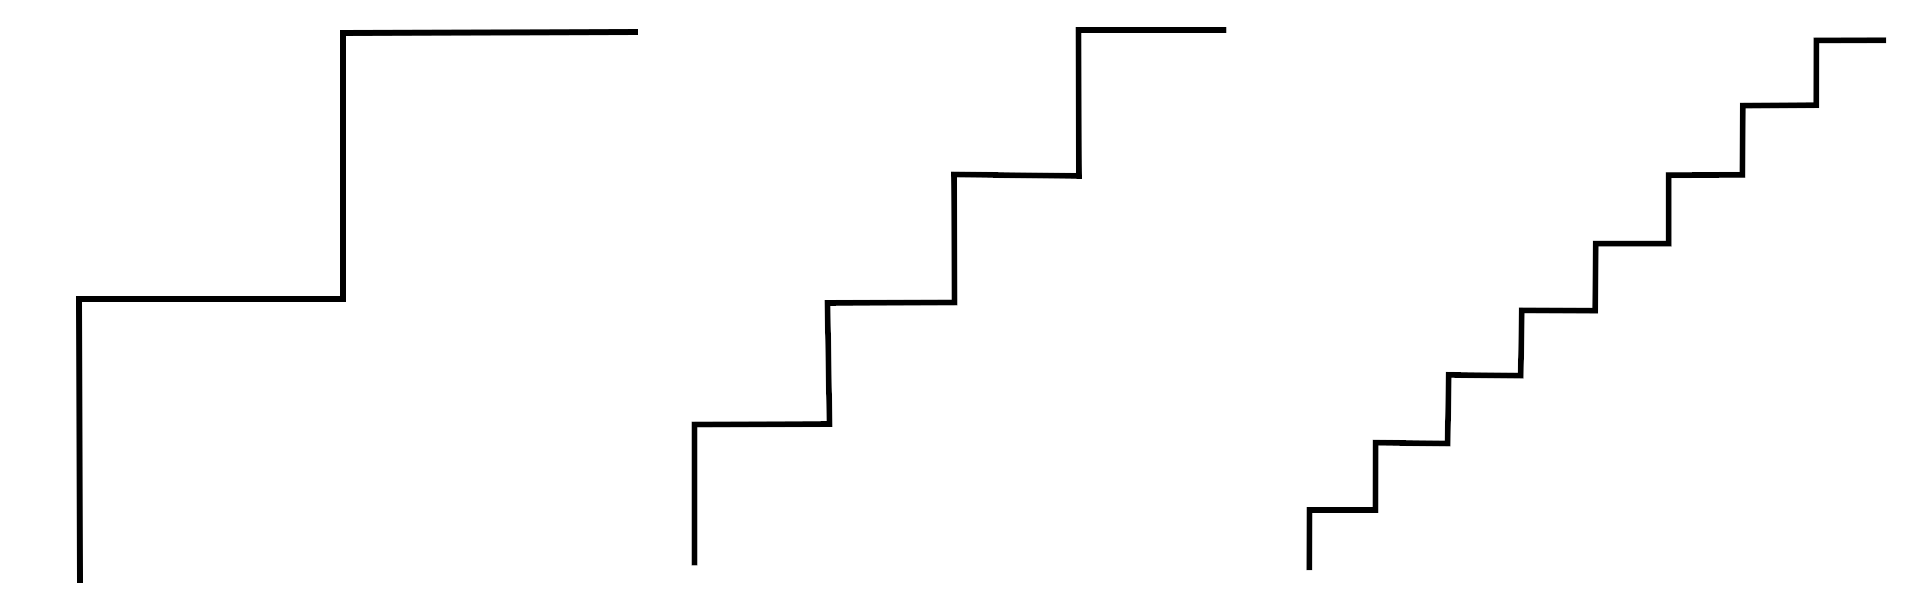
\includegraphics[height=8em]{\CWD/degraus_k123}
\end{center}
\end{figure}

Júlia notou que sua formiga demora 2 segundos para subir um segmento qualquer, independente do seu tamanho.
 Ela leva 1 segundo para percorrer um segmento horizontal, e apenas meio segundo para descer um segmento, qualquer que seja o seu tamanho.
 A formiga já está brincando há $N$ segundos, e é hora de dar comida para ela.
 Mas Júlia está sem óculos, e precisa de você para alimentar Fininha.
 Você pode dizer exatamente onde está a formiga agora?

\section*{Entrada}

A entrada contém apenas uma linha com os dois inteiros $K$ e $N$, separados por espaço, representando o número de transformações feitas por Júlia no brinquedo e há quantos segundos Fininha já está brincando.


\section*{Saída}

Escreva na saída dois números racionais separados por espaço, contendo as coordenadas $x$ e $y$ da posição de Fininha no segundo $N$.
 Considere que o ponto mais baixo do brinquedo
posicionado está na origem (ponto $(0, 0)$), e que o brinquedo termina na posição $(1, 1)$, onde Fininha começa a descer.

Essas posições não mudam com as transformações feitas.
 Como a posição de Fininha pode não ser inteira, escreva cada coordenada como uma fração irredutível da forma $a/b$ caso $b$ seja diferente de $1$.


\section*{Restrições}

$$0 \leq K \leq 40$$
$$0 \leq N \leq 10^{18}$$

\section*{Exemplos}
\exemplo
